\subsection{Task 1: Degree distribution}

\subsubsection{Description}
We conduct 5 experiments on large scale graph data(all with more than 1 million nodes). The details of each dataset is as follows: \\

\begin{center}
\begin{tabular}{| c | c | c |}
    \hline
    name & nodes & edges \\ \hline
    Roadnet-ca & 1,965,206 & 5,533,214 \\ \hline
    Roadnet-PA & 1,088,092 & 3,083,796 \\ \hline
    Roadnet-TX & 1,379,917 & 3,843,320 \\ \hline
    wiki-Talk & 2,394,385 & 5,021,410 \\ \hline
    Youtube & 1,134,890 & 2,987,624 \\ \hline
\end{tabular}
\end{center}

\subsubsection{Detailed Plots}
Following(Figure \ref{t1:plot}) are the rank-frequency plots of each dataset, (a)(b) shows the in degree and out degree out Wikitalk. (c) is Roadnet-Ca. (d) is Roadnet-PA. (e) is Roadnet-TX. (f) is Youtube. 

{\bf Proof of Correctness:} For each dataset, we compare the plot with its original groundtruth plot if it has.\footnote{Stanford SNAP does not have degree distribution, KONECT has degress distribution}. They are almost the same. 

\paragraph{Wiki-Talk}
In the wiki-talk graph, it's directed. Each node represents a user, and an edge represents a user at least edited another user's talk page. Figure \ref{t1:wiki} shows the in and out degree of this dataset. We don't have official degree distribution plot for this dataset. We can observe {\bf power law} from this plot. 
\begin{figure}[!htbf]
\begin{center}
\begin{tabular}{c c}
     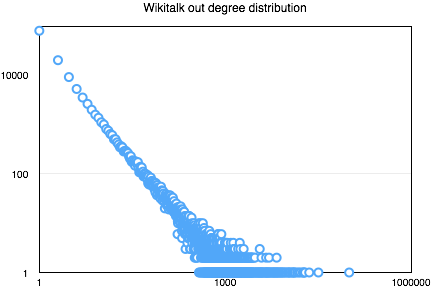
\includegraphics[width=0.3\textwidth]{FIG/t1_wiki_in.png} &
     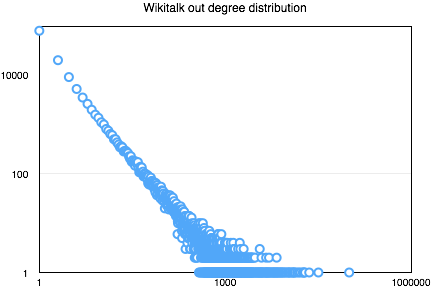
\includegraphics[width=0.3\textwidth]{FIG/t1_wiki_out.png} \\
    (a) & (b) \\
\end{tabular}
\caption{In degree distribution (a) and out degree distribution (b) of Wikitalk.}
\label{t1:wiki}
\end{center}
\end{figure}

\paragraph{Roadnet-CA}
Roadnet-CA is un undirected graph. Each node represents an intersection of road and edge is the road segments between two road intersections. Figure \ref{t1:ca}(a) shows our plot of degree distribution, Figure \ref{t1:ca}(b) is the original degree distribution of the dataset. We can see that they are the same. There is no obvious power law.
\begin{figure}[!htbf]
\begin{center}
\begin{tabular}{c c}
     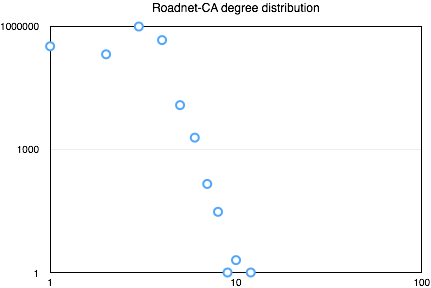
\includegraphics[width=0.3\textwidth]{FIG/t1_ca.png} & 
     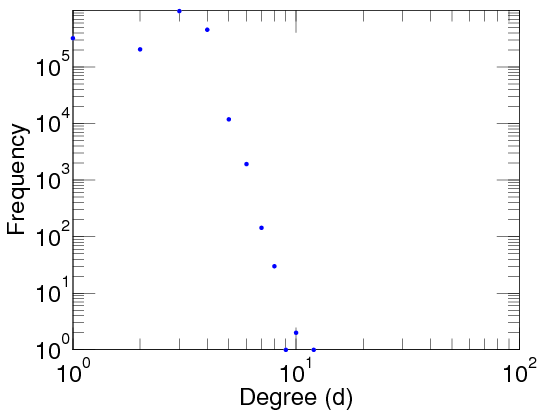
\includegraphics[width=0.3\textwidth]{FIG/t1_ca_truth.png}\\
    (a) & (b)\\
\end{tabular}
\caption{(a)Roadnet-CA (b) official degree distribution of Roadnet-CA}
\label{t1:ca}
\end{center}
\end{figure}


\paragraph{Roadnet-TX}
Roadnet-TX is un undirected graph. Each node represents an intersection of road and edge is the road segments between two road intersections. Figure \ref{t1:tx}(a) shows our plot of degree distribution, Figure \ref{t1:tx}(b) is the original degree distribution of the dataset. We can see that they are the same. There is no obvious power law.
\begin{figure}[!htbf]
\begin{center}
\begin{tabular}{c c}
     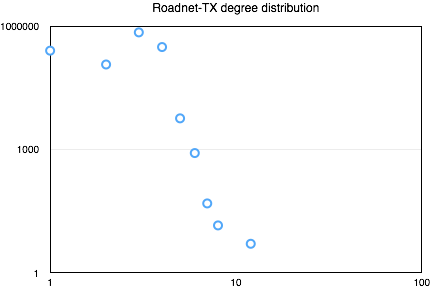
\includegraphics[width=0.3\textwidth]{FIG/t1_tx.png} & 
     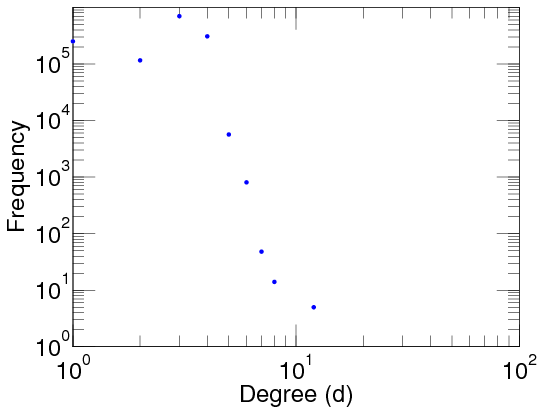
\includegraphics[width=0.3\textwidth]{FIG/t1_tx_truth.png}\\
    (a) & (b)\\
\end{tabular}
\caption{(a)Roadnet-TX (b) official degree distribution of Roadnet-TX}
\label{t1:tx}
\end{center}
\end{figure}

\paragraph{Roadnet-PA}
Roadnet-pa is un undirected graph. Each node represents an intersection of road and edge is the road segments between two road intersections. Figure \ref{t1:pa}(a) shows our plot of degree distribution, Figure \ref{t1:pa}(b) is the original degree distribution of the dataset. We can see that they are the same. There is no obvious power law.
\begin{figure}[!htbf]
\begin{center}
\begin{tabular}{c c}
     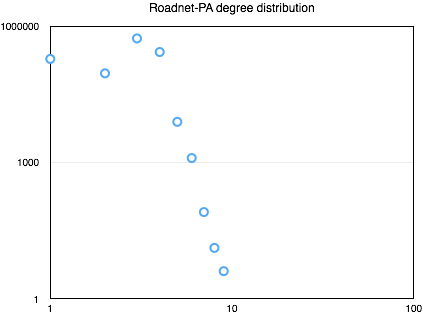
\includegraphics[width=0.3\textwidth]{FIG/t1_pa.png} & 
     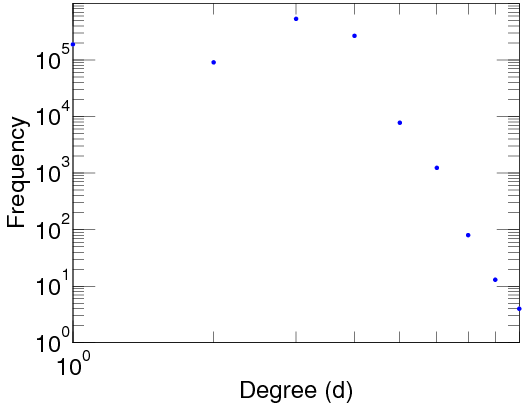
\includegraphics[width=0.3\textwidth]{FIG/t1_pa_truth.png}\\
    (a) & (b)\\
\end{tabular}
\caption{(a)Roadnet-pa (b) official degree distribution of Roadnet-pa}
\label{t1:pa}
\end{center}
\end{figure}

\paragraph{Youtube}
Youtube is an undirected graph, each node is a user in youtube.com, an edge represents they are friends. Figure \ref{t1:youtube}(a) shows our plot of the dataset, Figure \ref{t1:youtube}(b) is the official degree distribution of the dataset. We can see that they are exactly the same and there exhibits {\bf power law}.
\begin{figure}[!htbf]
\begin{center}
\begin{tabular}{c c}
     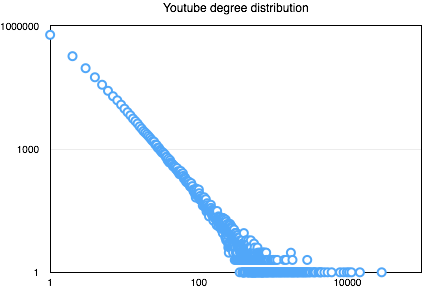
\includegraphics[width=0.3\textwidth]{FIG/t1_youtube.png} & 
     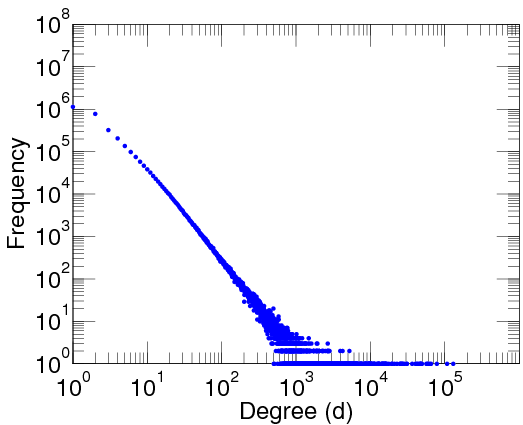
\includegraphics[width=0.3\textwidth]{FIG/t1_youtube_truth.png}\\
    (a) & (b)\\
\end{tabular}
\caption{(a)Youtube (b) official degree distribution of Youtube}
\label{t1:youtube}
\end{center}
\end{figure}

\subsubsection{Observation}
As we can observe, that most \emph{social network} exhibit perfect power law in degree distribution. It aligned with our intuition. While for the series of Roadnet dataset, we can not observe obvious power law. So maybe we can conclude that not all graphs have power law property in it. Some datasets like roadnet, involves a lot of human design, is less \emph{chaotic} than ordinary graphs.